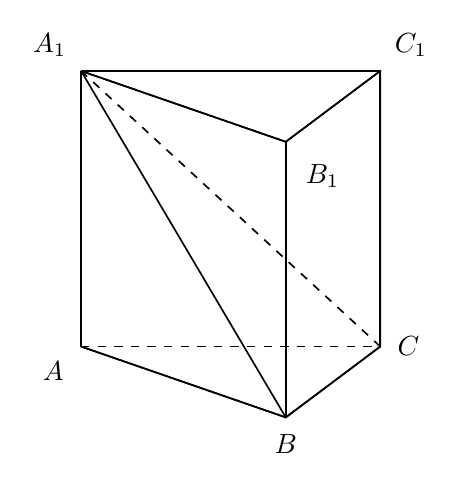
\begin{tikzpicture}[x=1cm,y=1cm,line width=.6pt,font=\normalsize,
geometry edge/.style={solid,line width=.6pt},
geometry label/.style={font=\normalsize,inner sep=2pt}]
% prism: vertical laterals, top/bottom triangles, plus A1B and A1C
\coordinate (A) at (0,0);
\coordinate (B) at (2.6,-0.9);
\coordinate (C) at (3.8,0);
\coordinate (A1) at (0,3.5);
\coordinate (B1) at (2.6,2.6);
\coordinate (C1) at (3.8,3.5);
% solid prism outline + top/bottom
\draw[geometry edge] (A1) -- (C1) -- (C) -- (B) -- (A) -- (A1);
\draw[geometry edge] (B1) -- (B);
\draw[geometry edge] (C1) -- (C);
\draw[geometry edge] (A1) -- (B1) -- (C1);
\draw[geometry edge] (A) -- (B) -- (C);
\draw[geometry edge] (B1) -- (C1);
\draw[geometry edge] (A1) -- (B1);
% interior plane A1BC
\draw[geometry edge] (A1) -- (B);
\draw[geometry edge,dashed] (A1) -- (C);
\draw[geometry edge,dashed] (A) -- (C);
\node[geometry label,above left,xshift=-3pt,yshift=3pt] at (A1) {$A_{1}$};
\node[geometry label,above right,xshift=3pt,yshift=3pt] at (C1) {$C_{1}$};
\node[geometry label,below right,xshift=5pt,yshift=-6pt] at (B1) {$B_{1}$};
\node[geometry label,below left,xshift=-4pt,yshift=-3pt] at (A) {$A$};
\node[geometry label,below,yshift=-4pt] at (B) {$B$};
\node[geometry label,right,xshift=4pt] at (C) {$C$};
\end{tikzpicture}
